%datasheets ne555, 2n2222, octave
\paragraph{}
En este apartado se expondr\'a el diseño del transmisor, los c\'alculos matem\'aticos necesarios, la simulaci\'on por ordenador y los resultados pr\'acticos.
El transmisor está diseñado para generar una modulación ASK y emitir a una frecuencia de unos \SI{30}{\mega\hertz}. La frecuencia de emisión es sintonizable con la del receptor por medio de un condensador de capacidad variable.
\paragraph{}
En la figura \ref{fig:tx} se puede observar el esquema eléctrico del transmisor.
El principio de funcionamiento del transmisor es un oscilador basado en un par resonante $LC$, el cual fija la frecuencia de emisión. 
La oscilaci\'on se genera realizando un bucle de realimentación positiva, donde el transistor NPN juega el papel de elemento activo de amplificación. 
El circuito tanque $LC$ es el filtro que permite que en cada iteración del bucle se amplifique la frecuencia deseada. A su vez, el condensador de realimentación genera la realimentación positiva, sumando una fracción de la salida con la señal de entrada, que en este caso es el propio ruido generado por el circuito.
El circuito se diseña de forma que se disipe la mayor potencia posible, con el fin de que la señal recorra la mayor distancia alcanzable. 
\paragraph{}
Por otra parte, el cicuito permite modular la señal portadora eléctricamente cortando y produciendo la oscilación en función de las variaciones de la señal moduladora. Esto es posible gracias al segundo transistor PNP, el cual trabaja en corte y saturaci\'on y corta el paso de corriente general del circuito.
% Esto se realiza por medio de un oscilador Colpitts en base común sintonizado a la frecuencia de emisión y que a su vez es mezclado con una señal de onda cuadrada generada por el chip integrado NE555.
% La señal de onda cuadrada generada por el NE555, es modulada en frecuencia, por dos pulsadores, produciendo dos diferentes canales digitales de salida.
El esquema completo del transmisor se expone en la figura \ref{fig:tx}.

\begin{figure}[h]
    \centering
    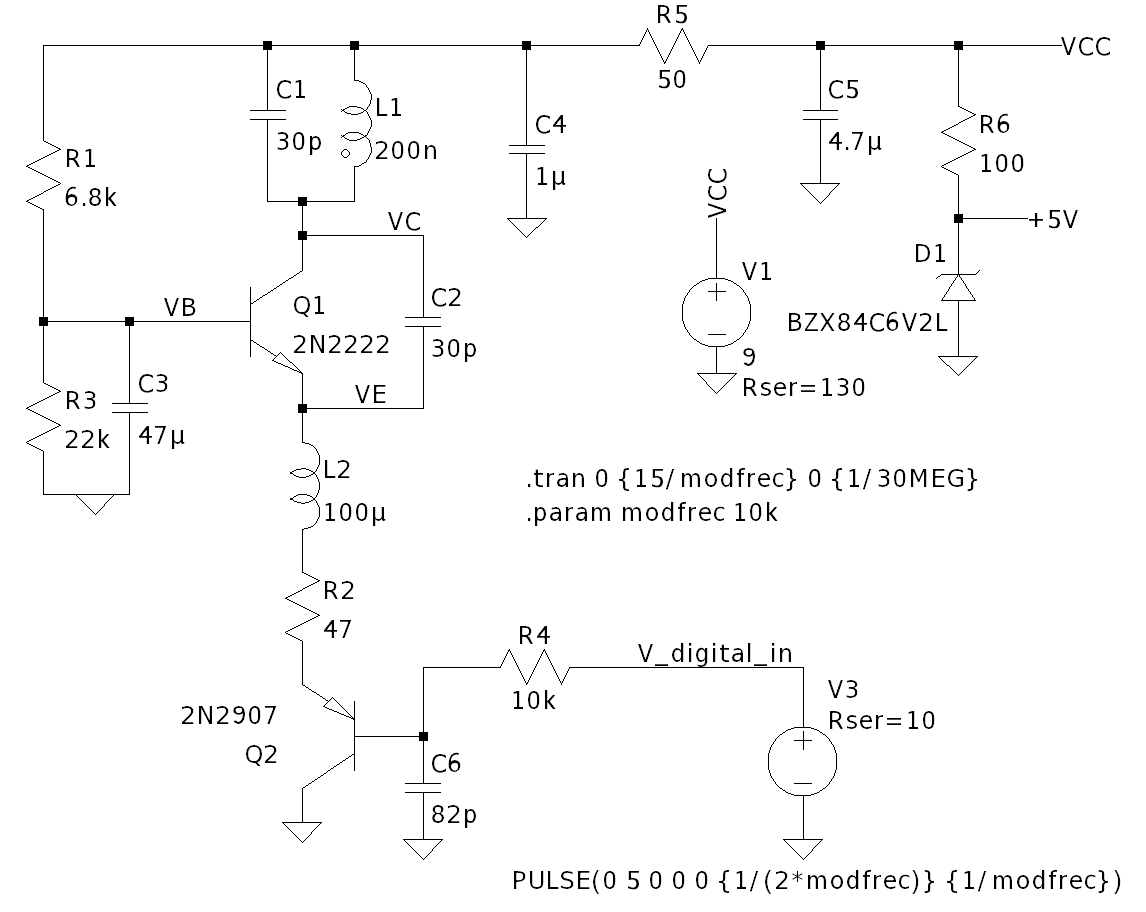
\includegraphics[scale=1, width=1\textwidth]{transmisor}
    \caption{Esquema el\'ectrico del transmisor}
    \label{fig:tx}
\end{figure}

\paragraph{Diseño del oscilador}
\paragraph{Polarizaci\'on} %IGUAL Y MENCIONANDO EL TRANSISTOR PNP EN CORTE APROX 0.2 V DESPRECIABLE.
\paragraph{}
Primeramente, se debe fijar el punto de operación deseado. Se deben tener encuenta dos cosas: la zona de trabajo del transistor y la potencia del circuito. La zona de trabajo debe ser activa directa, pues para producir la oscilación, el bucle de realimentación positiva debe tener la etapa de amplificación proporcionada por el transistor. La potencia del circuito, junto a la frecuencia de diseño, acotan el modelo de transistor que se ajusta a las necesidades del circuito.
\paragraph{}
En primer lugar, se necesita un transistor con una frecuencia de transición $f_t > \SI{30}{\mega\hertz}$. 
A parte de esto, el parámetro $I_{Cmax}$ debe ser suficiente para proporcionar la potencia deseada sin deteriorarse. Se elige un transistor 2N2222, cuya $f_t > \SI{30}{\mega\hertz}$ e $I_{Cmax} = \SI{0.6}{\ampere}$. Adem\'as, se fija una $V_{CC} = \SI{9}{\volt}$ el cual ser\'a el mayor valor que pueda tener, pero esto no implica que el transmisor pueda funcionar con tensiones de alimentaci\'on inferiores. Se opta por limitar a $Ic = \SI{100}{\milli\ampere}$, que supondr\'a una potencia de aproximadamente $I_C \cdot V_{CC} = \SI{0.72}{\watt}$ y $V_{CE} = \frac{V_{CC}}{2} = \SI{4.5}{\volt}$, condici\'on necesaria para trabajar en activa directa con el mayor rango de margen de distorsi\'on. 
\paragraph{}
Adicionalmente, se obtienen los par\'ametros necesarios de la hoja de características del 2N2222\footnote{ON Semiconductor. (2016). \textit{2N2222A: Small Signal Transistor Datasheet}. Recuperado de \url{https://www.onsemi.com/pdf/datasheet/2n2222a-d.pdf}.}.
Se conoce $h_{FEmax} \approx 300$ de la hoja de datos, aunque, medido con un mult\'imetro, se obtiene el valor $h_{FE} = 280$, por lo que se utilizar\'a este \'ultimo.
\paragraph{}
En lugar de repetir el cálculo que se hizo para seleccionar el valor de las resistencias de polarización, se opta por verificar si los valores elegidos satisfacen las imposiciones. 
Esto es debido a que, una vez se realizaron los c\'alculos, los valores de las resistencias de polarizaci\'on fueron aproximados a valores comerciales para la construcci\'on del dispositivo. De esta forma, se obtinene una comprobaci\'on doble. Adem\'as, en todo el proceso se considera despreciable la ca\'ida de tensi\'on en el transistor PNP, la cual es de unos \SI{.2}{\volt} en condici\'on de saturaci\'on.
\paragraph{}
Se utiliza equivalente de Thevenin para las resistencias en paralelo. En la malla que aparece se obtiene:
$$V_{th} - 0.7 - I_c \cdot R_e = I_b \cdot R_{th}$$
Siendo:
\renewcommand{\arraystretch}{1.5}
\[
\begin{array}{rl} 
      \begin{array}{l}
	 V_{th} = \frac{V_{CC} \cdot R_2}{R_1+R_2} \\
	 R_{th} = \frac{R_1 \cdot R_2}{R_1+R_2}
      \end{array}
      &
      \begin{array}{l}
	 I_b \cdot h_{FE}= I_c \\
	 h_{FE} = 280
      \end{array}
\end{array}
\]
Se obtienen $I_c$ y $V_{CE}$ con las siguientes dos ecuaciones sustituyendo los valores correspondientes:
\begin{align*}
   R_1=\SI{6.8}{\kilo\ohm} \quad R_2=\SI{22}{\kilo\ohm} \quad &R_E=\SI{47}{\ohm} \quad V_{CC} = \SI{9}{\volt} \\
   I_c \cdot \left( R_E+ \frac{R_{th}}{h_{FE}}\right) &= V_{th} - 0.7 \\
   V_{CC} = V_{CE} &+ I_C \cdot R_E
\end{align*}
\begin{equation}
   V_{CE}= \SI{4.57}{\volt} \quad I_C = \SI{94.2}{\milli\ampere}
\end{equation}
\paragraph{}
Una vez calculado el punto de operaci\'on, se obtienen los par\'ametros h\'ibridos en base com\'un siguiendo la metodolog\'ia expuesta en el apartado \ref{sec:teo_transistor}. En primer lugar, se deben calcular los parámetros híbridos en emisor común a partir de los resultados obtenidos en el punto de operación, utilizando las ecuaciones \ref{eq:h_param1} y \ref{eq:h_param2}. En segundo lugar, se deben aplicar las transformaciones indicadas en la ecuaci\'on \ref{eq:h_conversion}. Adem\'as se debe calcular el dato $V_{AF}$ con ayuda de la hoja de datos del transistor, en este caso el dato se obtuvo como una media del rango de valores proporcionado. El resultado del c\'alculo de los par\'ametros es el siguiente:
\begin{equation}
   \label{eq:result_pol1}
V_{AF} = \frac{I_{Cdata}}{h_{OEdata}} =\frac{\SI{1}{\milli\ampere}}{\SI{6}{\micro\siemens}} =  \SI{50}{\volt} 
\end{equation}
\begin{equation}
   \label{eq:result_pol2}
%\[
\begin{array}{rl} 
      \begin{array}{l}
	 h_{ib} =  \SI{7.4}{\ohm} \\
	 h_{fb} =  -0.996
      \end{array}
      &
      \begin{array}{l}
	 h_{rb} =  0.014 \\
	 h_{ob} =  \SI{6.7}{\micro\siemens}
      \end{array}
\end{array}
%\]
\end{equation}

\begin{figure}[h]
    \centering
    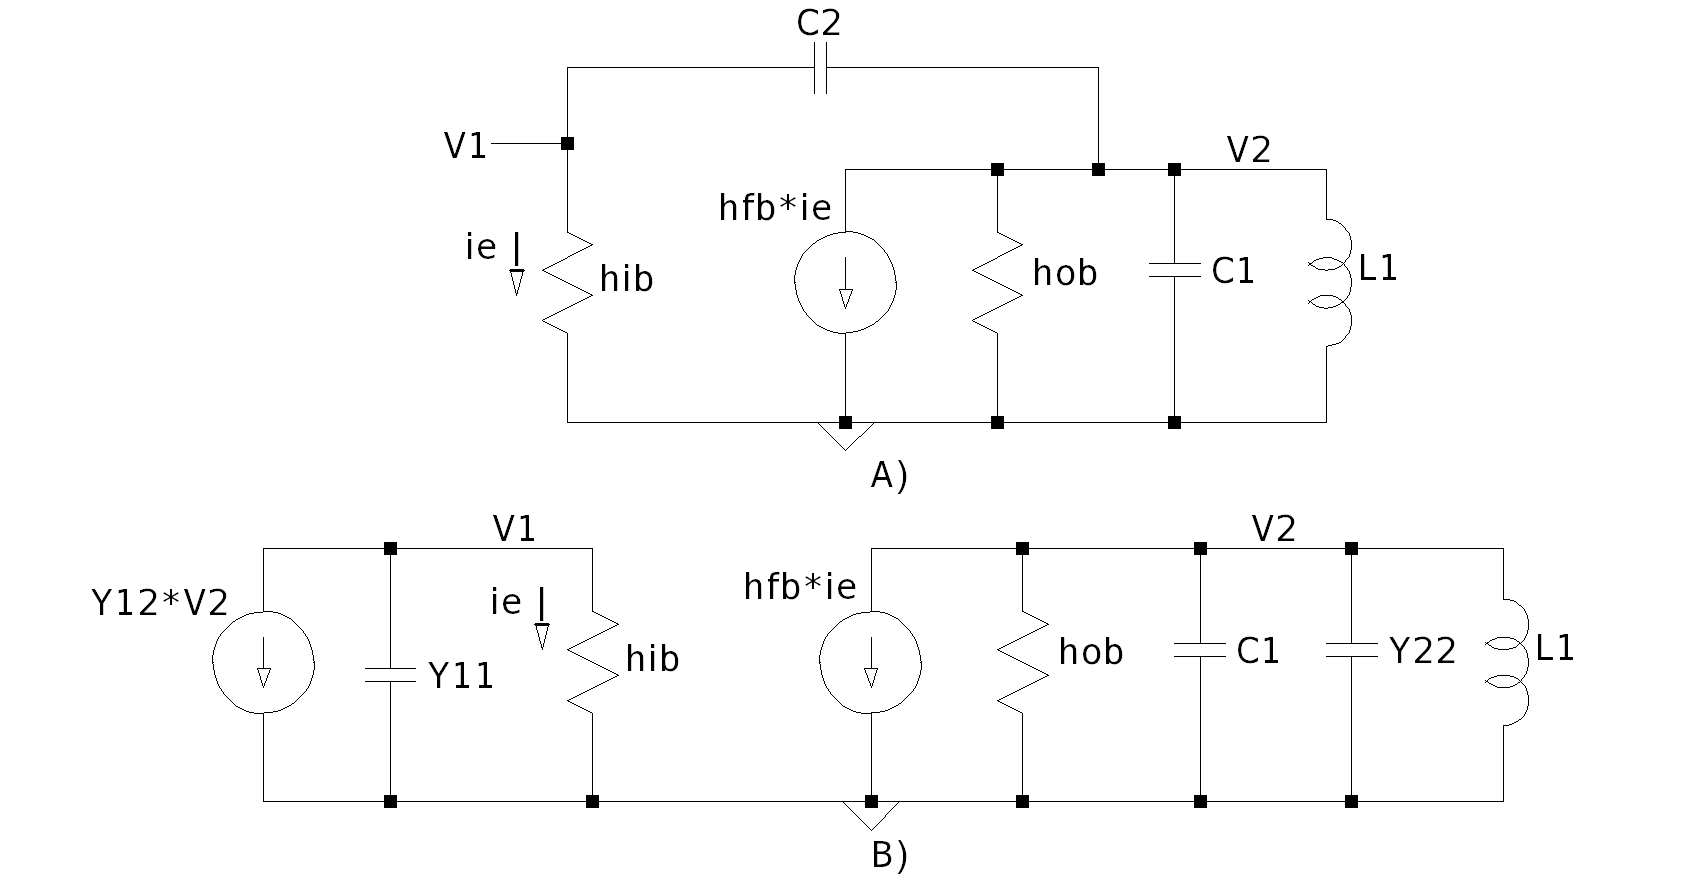
\includegraphics[scale=1, width=.8\textwidth]{small_signal_tx}
    \caption{A) Modelo en pequeña señal del bucle de oscilación para frecuencias medias B) Modelo en pequeña señal del oscilador sustituyendo el condensador de realimentación $C_1$ por su equivalente en parámetros $Y$}
    \label{fig:ss_tx}
\end{figure}

\paragraph{Modelo en pequeña señal} %ANADIR LOS CALCULOS DE LA INDUCTANCIA APROX 200N SEGUN INTERESE. 
\paragraph{}
El objetivo de este modelo es el cálculo de la frecuencia de resonancia del oscilador. En la figura \ref{fig:ss_tx} se muestra el modelo en pequeña señal del oscilador para frecuencias intermedias, en torno a la frecuencia de oscilaci\'on. El bucle de oscilaci\'on se trata de una realimentación paralelo-paralelo, por lo que se representa el condensador de realimentación $C_1$ como su equivalente en par\'ametros $Y$. El valor de dichos par\'ametros son:
\[
\begin{array}{rl} 
      \begin{array}{l}
	 Y_{11} = \frac{i_1}{v_1}|_{v_2 = 0} = s \cdot C_2 \\
	 Y_{12} = \frac{i_1}{v_2}|_{v_1 = 0} = -s \cdot C_2 
      \end{array}
      &
      \begin{array}{l}
	 Y_{21} = \frac{i_2}{v_1}|_{v_2 = 0} = -s \cdot C_2 \\
	 Y_{22} = \frac{i_2}{v_2}|_{v_1 = 0} = s \cdot C_2 
      \end{array}
\end{array}
\]
\paragraph{}
Se deben tener en cuenta ciertas consideraciones previas como consecuencia del an\'alisis del esquema B) en la figura \ref{fig:ss_tx}. La realimentaci\'on es positiva en el momento que $Y_{12}<0$ y $h_{fb}<0$ por lo que $V_2>0$. El modelo que se muestra corresponde a frecuencias intermedias en torno a la de oscilaci\'on. Para frecuencias bajas, la impedancia de $C_2$ tendrá un valor tan alto que corta la realimentación, siguiendo el esquema A) figura \ref{fig:ss_tx}. 
Para frecuencias altas, la impedancia de $C_2$ tendr\'a un valor tan bajo que supondr\'a un cortocircuito a tierra para la corriente de realimentaci\'on, por lo que $ie = 0 \unit{\ampere}$.
\paragraph{}
Se calcula la frecuencia de resonancia, en base al modelo B) de la figura \ref{fig:ss_tx}. Siguiendo el criterio de Barkhausen, la frecuencia de resonancia se corresponde con la única con desfase $\angle A_l(f_0) = \SI{180}{\degree}$ a lo largo del bucle y una magnitud $|A_l(f_0)|\ge 0$. Se obtiene la funci\'on de transferencia de la ganancia en lazo abierto.
Siguiendo el modelo general de la realimentaci\'on (ecuaci\'on \ref{eq:feedback} aplicada al esquema B) de la figura \ref{fig:ss_tx}), se calcula: 
\begin{equation}
f = Y_{12} = -s \cdot C_2
\end{equation}
\paragraph{}
Se muestra el desarrollo para el c\'alculo de $A = \frac{V_2}{i_E}$:
\[
\begin{array}{rl} 
      \begin{array}{l}
   \frac{i_E}{V_1} = Y_{T1} = s\cdot C_2 + \frac{1}{h_{ib}} \\
   \frac{i_e}{V_{1}} = \frac{1}{h_{ib}} \\
   i_E = Y_{T1} \cdot i_e \cdot h_{ib}
      \end{array}
      &
      \begin{array}{r}
   \frac{V_2}{h_{fb}\cdot i_e} = {Y_{T2}}^{-1} \\
   Y_{T2} = s\cdot C_2 + s\cdot C_1 + \frac{1}{s\cdot L_1} + h_{ob} \\
   V_2 = \frac{h_{fb}\cdot i_e}{Y_{T2}} 
      \end{array}
\end{array}
\]
\begin{equation}
   A = \frac{-h_{fb}}{Y_{T1} \cdot Y_{T2} \cdot h_{ib}} 
\end{equation}
\paragraph{}
Se calcula la ganancia en lazo abierto como $A_l = A \cdot f$ y sustituyendo los valores de $Y_{T1}$ e $Y_{T2}$:
\begin{equation}
   \label{eq:Al_tx}
   A_l = \frac{h_{fb} \cdot C_1 \cdot s^2}{ \left( C_2+C_1 \right) \left( s \cdot h_{ib} \cdot C_2 + 1\right) \left( s^2 + s \cdot \frac{h_{ob}}{C_1 + C_2} + \frac{1}{(C_1 + C_2)\cdot L_1}\right) }
\end{equation}
\paragraph{}
De la expresi\'on obtenida en la ecuaci\'on \ref{eq:Al_tx}, se deduce el siguiente an\'alisis. 
En primer lugar, se analiza el desfase, el cual a bajas frecuencias es \SI{0}{\degree}, debido a la suma de los \SI{180}{\degree} del cero doble junto a los \SI{180}{\degree} de $h_{fb} < 0$. A su vez, el polo cuadr\'atico introduce un desfase de \SI{-180}{\degree}, al que se llega de forma r\'apida debido al bajo valor del coeficiente de amortiguaci\'on, el cual se obtiene como:$$\zeta = \frac{h_{ob} \cdot \sqrt{(C_1+C_2) \cdot L_1}}{(C_1+C_2) \cdot 2} = \num{2.9e-4}$$
Adem\'as, se añaden los \SI{-90}{\degree} del polo simple, el cual, se considera no dominante por su alto valor: $s = \frac{-1}{h_{ib} \cdot C_2} = \SI{4.5e9}{\radian\per\second}$. 
Consecuentemente, se obtiene que la frecuencia de resonancia con desfase \SI{180}{\degree} es aproximadamente igual que la frecuencia de resonancia del polo cuadrático, es decir:
$$\omega_0 = \SI{1.925e8}{\radian\per\second}$$ 
Por lo que:
\begin{equation}
   f_0 = \frac{\omega_0}{2\cdot\pi} = \SI{30.63}{\mega\hertz}
\end{equation}
\paragraph{Fabricaci\'on de la inductancia del circuito tanque}
\paragraph{}
La inductancia del circuito tanque $LC$, es construida a mano para facilitar la radiación al medio. Esta inductancia será el elemento principal de radiación.
En contraparte, las inductancias comerciales en su fabricación se centran en tener un reducido tamaño y evitar radiación al medio, produciendo bajas interferencias. Este hecho es contrario al objetivo que se busca.
\paragraph{}
La expresión de inductancia $L$ de la bobina en función de sus parámetros físicos se desarrolla de la siguiente forma\footnote{Kulkarni, S. V., \& Khaparde, S. A. (2004). \textit{Transformer Engineering: Design and Practice} (Capítulo 1: Transformer Fundamentals). Indian Institute of Technology, Bombay, Mumbai, India.}:
\paragraph{}
Por un lado se tiene la definici\'on de inductancia ($L$), es decir, la variación del flujo con respecto a la variación de corriente por un bobinado: 
\begin{equation}
   \label{eq:def_inductance}
   L = N \cdot \frac{d\theta}{di}
\end{equation}
\paragraph{}
Por otro lado, se aplica la ley de Amp\`ere para un único bobinado:
\begin{equation}
   \label{eq:def_ampere}
   \mathcal{R} = N \cdot \frac{di}{d\theta} \quad \quad
   \mathcal{R} = \frac{l}{\mu \cdot A_c}
\end{equation}
\paragraph{}
Combinando las ecuaciones \ref{eq:def_ampere} y \ref{eq:def_inductance}, se obtiene la expresi\'on para el c\'alculo de la inductancia:
\begin{equation}
   \label{eq:def_inductance2}
   L = \frac{N^2 \cdot \mu_0 \cdot \left(\frac{d}{2} \right)^2 \cdot \pi}{l}
\end{equation}
\paragraph{}
En este caso, los par\'ametros medidos en la inductancia fabricada son: $N = 8$, $\mu = \mu_0$, $d = \SI{8}{\milli\metre}$ y $l = \SI{9}{\milli\metre}$. El resultado de la aplicaci\'on de la ecuaci\'on \ref{eq:def_inductance2} con los par\'ametros medidos resulta en: $$L_1 = \SI{450}{\nano\henry}$$

% \paragraph{Diagrama de Bode}
% \paragraph{}
% A continuación, se esboza el diagrama de Bode de la expresi\'on de la ganancia de lazo abierto (ecuaci\'on \ref{eq:Al_tx}) para los valores obtenidos en el apartado de polarizaci\'on (ecuaciones \ref{eq:result_pol1} y \ref{eq:result_pol2}) junto con los siguientes valores de los elementos: 
% $$ L_1 = \SI{450}{\nano\henry} \quad C_1=\SI{30}{\pico\farad} \quad C_2=\SI{30}{\pico\farad} $$
% \begin{figure}[h]
%     \centering
%     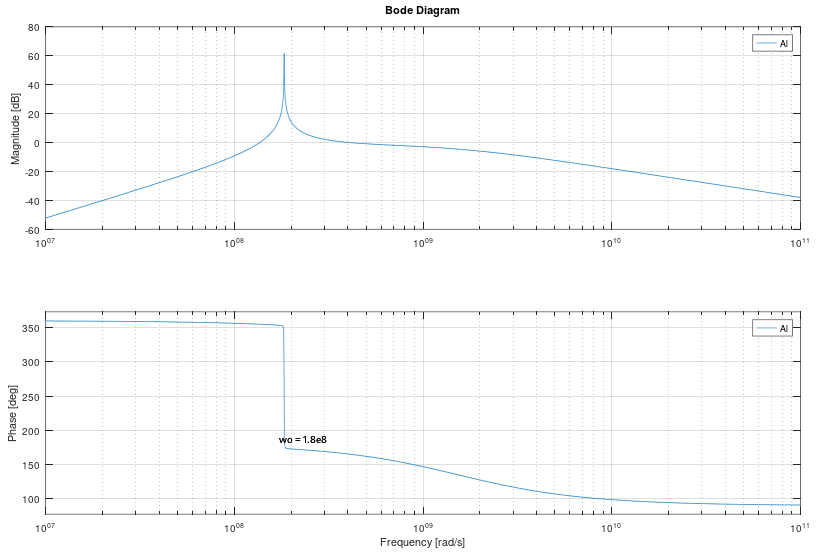
\includegraphics[scale=1, width=.8\textwidth]{bode_tx}
%     \caption{Diagrama de Bode de la ganancia en lazo abierto del oscilador $A_l$ para frecuencias intermedias}
%     \label{fig:bode_tx}
% \end{figure}
% \paragraph{}
% La obtenci\'on del diagrama de Bode se ha realizado con ayuda del programa de c\'alculo computacional Octave. Los \textit{scripts} utilizados se encuentran el el directorio octave del proyecto de GitHub\footnote{\textit{https://github.com/josegu05/tfg2}}.

\paragraph{}
\paragraph{Regulador de tensi\'on: carril de +\SI{5}{\volt}}
\paragraph{}
Para conseguir independencia de la fuente de alimentaci\'on general con respecto de la alimentaci\'on del microcontrolador de la parte digital, se añade un pequeño regulador de tensión formado por una resistencia, un diodo \textit{zener} y un condensador. 
Este método también actúa a modo de protección contra posibles picos de tensión de la fuente principal, protegiendo el microcontrolador, además de proporcionar estabilidad, mejorando su rendimiento.
En contraparte, el regulador, al tener un diseño simple, sufre de un excesivo consumo estático, siendo este, el mayor calculado independientemente del consumo de su carga.
El cálculo del valor de la resistencia de protección se realiza según las necesidades de potencia. Se tiene:
\begin{align*}
   P_{zener_{max}} &= \SI{.5}{\watt} \\
   V_{CC_{max}} &= \SI{9}{\volt} \\
   I_{AVR_{max}} &\approx \SI{50}{\milli\ampere} \\
   P_{load_{max}} &= V_{zener} \cdot I_{AVR_{max}} < P_{zener_{max}}\\
   P_{R_{Lim}} &= (V_{CC_{max}} - V_{zener}) \cdot I_{AVR_{max}}
\end{align*}
\begin{equation}
   R_{Lim} = \SI{78}{\ohm}
\end{equation}
\paragraph{}
El valor de $R_{Lim}$ obtenido, se trata del m\'inimo para satisfacer los requisitos impuestos, pues $I_{AVR_{max}}$ se encuentra sobredimensionado. 
\paragraph{}
Empíricamente, en la figura \ref{fig:tx}, se usa $R_{Lim} = R_6 = \SI{100}{\ohm}$, aunque este valor puede ser aún mayor.
En cuanto a $C_5$, se usa un valor de $C_5 = \SI{4.7}{\micro\farad}$. Este valor se considera suficientemente alto como para estabilizar la tensi\'on y adem\'as suficientemente bajo como para que, al arranque del cicuito, cuando $C_5$ se encuentre descargado, no suponga un pico de corriente muy alto y prolongado para la fuente de alimentaci\'on.
La resistencia $R_5 = \SI{50}{\ohm}$ act\'ua de separador entre la parte de RF y digital. Además, se comporta como un filtro paso bajo, evitando que señales de RF se filtren hacia el microcontrolador.
\paragraph{} 
Por último, se hace referencia al transistor PNP. %en el esquema del transmisor (figura \ref{fig:tx}). 
Este transistor es utilizado como conmutador, de tal forma que, una señal digital activa o corta el paso de corriente por el circuito principal. La señal digital de inicio o corte es producida por el microcontrolador Atmega328p, y se desarrollará en el correspondiente apartado (apartado \ref{sec:des_digital_tx}).

\paragraph{}
\paragraph{Antena y transformador de impedancias} 
%CITAR TRANSFORMER BOOK
%CALCULOS: 
%Primero impedancia de salida del circuito sin bobina (usada de primario), y generador a la frecuencia de resonancia. 
%segundo, modelo del transformador y transformacion de impedancias a cable de 1k aprox?
%simulacion de potencia disipada por la antena?
\paragraph{}
Para mejorar la eficiencia de radiación del transmisor, se debe garantizar la máxima transferencia de potencia de señal a la antena.
Para poder adaptar la impedancia de salida del circuito a la impedancia de la antena, se diseña un transformador como adaptador de impedancias. 
Se considera esta opción como la alternativa más sencilla de implementar, debido a que el circuito necesita una impedancia de salida bastante alta para poder producir la oscilación.
El método del transformador adapta las impedancias considerablemente bien, mediante un acople magnético, es decir, sin cargar el circuito.
\paragraph{}
El objetivo del diseño es calcular la relación del número de vueltas óptimo entre el primario y el secundario para mejorar la transferencia de potencia entre el transmisor y la antena. 
Para facilitar los cálculos, pues existen demasiados parámetros reales que se deben aproximar, se seguirá un modelo ideal sencillo del transformador. Esto es debido a que solo se busca mejorar el aspecto de la transmisión de potencia que se tiene de base.
Se sigue el siguiente modelo de relación de impedancias en un transformador\footnote{Kulkarni, S. V., \& Khaparde, S. A. (2004). \textit{Transformer Engineering: Design and Practice} (Capítulo 1: Transformer Fundamentals). Indian Institute of Technology, Bombay, Mumbai, India.}.

\paragraph{}
\begin{figure}[h!]
    \centering
    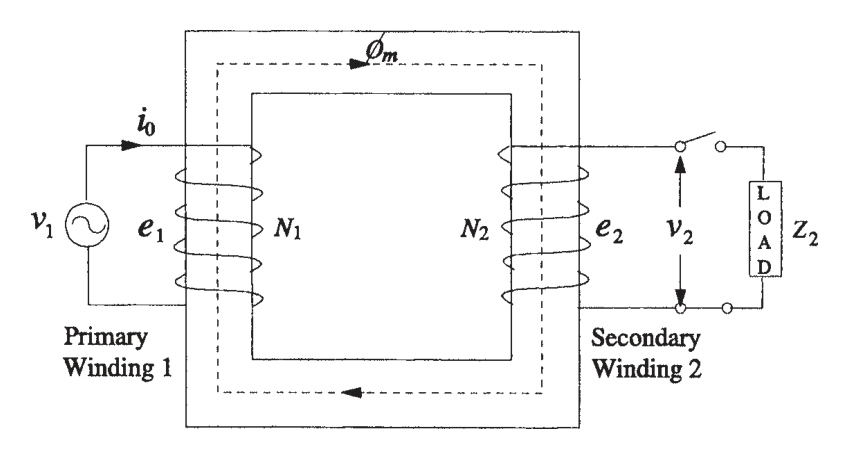
\includegraphics[scale=.7, width=.7\textwidth]{transformer2}
    \caption{Modelo de transformador ideal}
    \label{fig:transformer}
\end{figure}
\paragraph{}
Siguiendo el modelo de la figura \ref{fig:transformer}, se obtienen las siguientes relaciones:
\begin{align*}
   \frac{N_1}{N_2} = \frac{E_1}{E_2} &= \frac{V_1}{V_2} = \frac{I_2}{I_1} = n \\
   Z_1 &= V_1 \cdot I_1 \\
   Z_2 &= V_2 \cdot I_2 \\
\end{align*}
\begin{equation}
   \label{eq:transformer}
   \frac{Z_1}{Z_2} = n^2 
\end{equation}
%\equation
%	Np/Ns = n = V2/V1 .. n^2 = zp/zs
\paragraph{}
En particular para el diseño propio se debe calcular tanto la impedancia de salida del transmisor como la resistencia de radiación de la entena utilizada para la frecuencia de trabajo.
Se tiene que $Z_1 = h_{ob}^{-1}$ y que la impedancia de la antena es aproximadamente $Z_2 = R_{rad} = \SI{1}{\kilo\ohm}$.
Por lo tanto, se usa la ecuaci\'on \ref{eq:transformer} para obtener el ratio de vueltas óptimo siendo: $$ n = \sqrt{\frac{Z_1}{Z_2}} = 10 $$
Esta relación de vueltas óptima no es realizable, pues el bobinado primario se construye con ocho espiras. La relación de vueltas aproximada será de $ n = 8:1 $


\paragraph{Resultado de la simulaci\'on} %SIMULACION LTSPICE
%son 3 capturas una la de la oscilacion con las medidas de frecuencia.
%una general con varios ciclos de digitalin.
%otra del flanco de subida y bajada de digitalin con vout y vbe viendo como se corta el transistor.
\paragraph{}
En este apartado se muestra una simulación del circuito en función del tiempo de los puntos de interés del circuito. 
En la figura \ref{fig:sim_vc_vdig} se observa el $V_C$, que es la tensión que se aplicará en el transformador de impedancias a la antena, y $V_{digital}$, la señal moduladora que produce la modulación ASK. 
\begin{figure}[h]
    \centering
    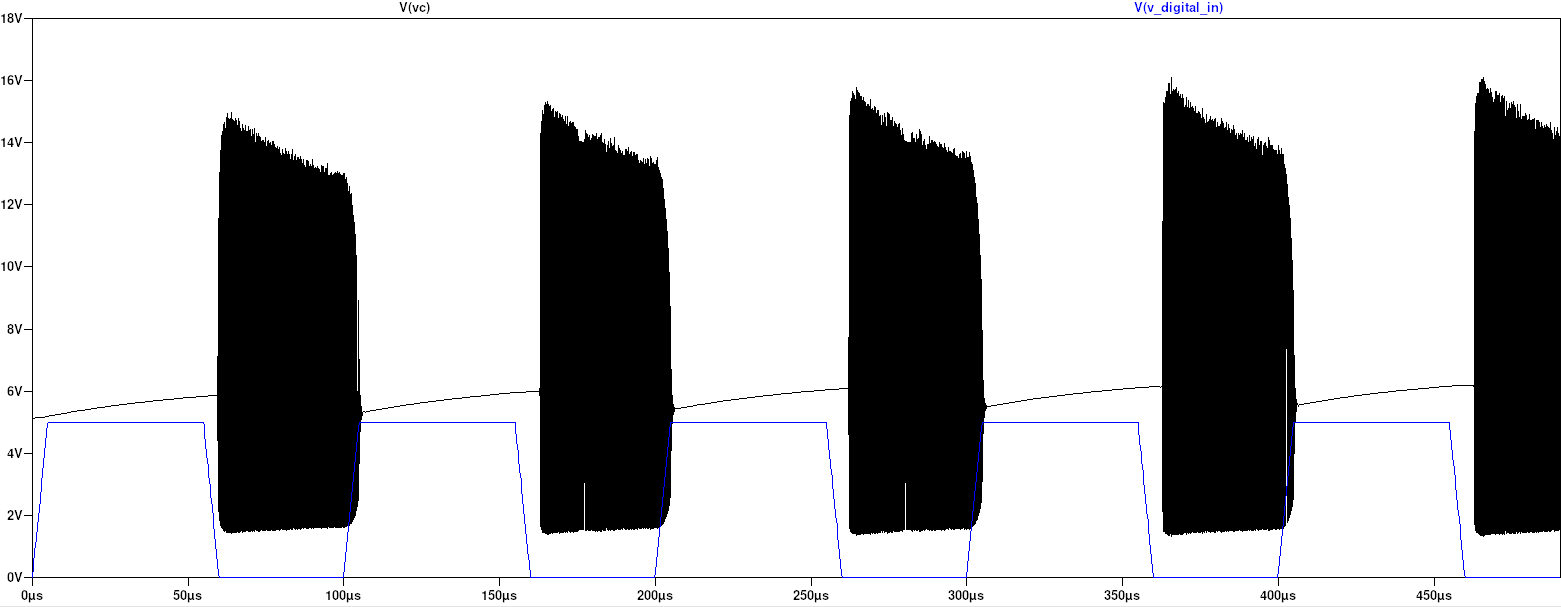
\includegraphics[scale=.8, width=.8\textwidth]{sim_vc_vdigital}
    \caption{Simulaci\'on de $V_C$ modulada por $V_{digital}$}
    \label{fig:sim_vc_vdig}
\end{figure}
\paragraph{}
En la figura \ref{fig:sim_fft} se observa la FFT de la señal $V_C$ de forma general, con un span de frecuencias alto. Por otro lado, en la figura \ref{fig:fft_vc_zoom} se muestra ampliada la frecuencia de trabajo, en la que se pueden observar los detalles de la modulación AM.
\paragraph{}
En la figura general de la FFT, al tratarse de una modulación ASK, se observa con acentuada potencia la señal moduladora en banda base. Además, esta señal posee una forma de onda cuadrada, por lo que su espectro se extiende ampliamente en el dominio de la frecuencia, aportando numerosos armónicos.
\paragraph{}
En la figura \ref{fig:fft_vc_zoom}, se observa el espectro de la modulación ampliado a la frecuencia de trabajo. Se sitúan cursores a la frecuencia de trabajo y los armónicos fundamentales a \SI{10}{\kilo\hertz}. Además, se pueden observar multitud de armónicos secundarios a distancias múltiplos de la frecuencia fundamental \SI{10}{\kilo\hertz}.
\begin{figure}[h!]
    \centering
    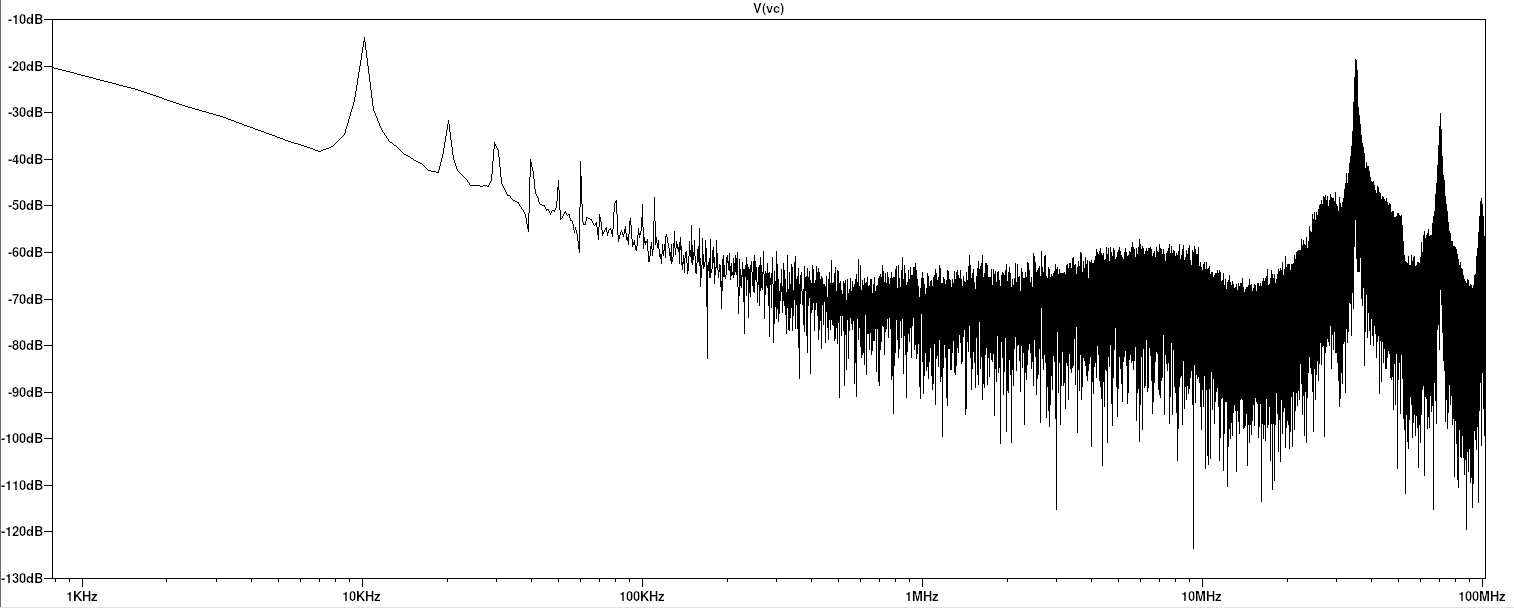
\includegraphics[scale=.8, width=.8\textwidth]{fft_vc}
    \caption{Simulaci\'on de la FFT de $V_C$ de forma general}
    \label{fig:sim_fft}
\end{figure}
\begin{figure}[h!]
    \centering
    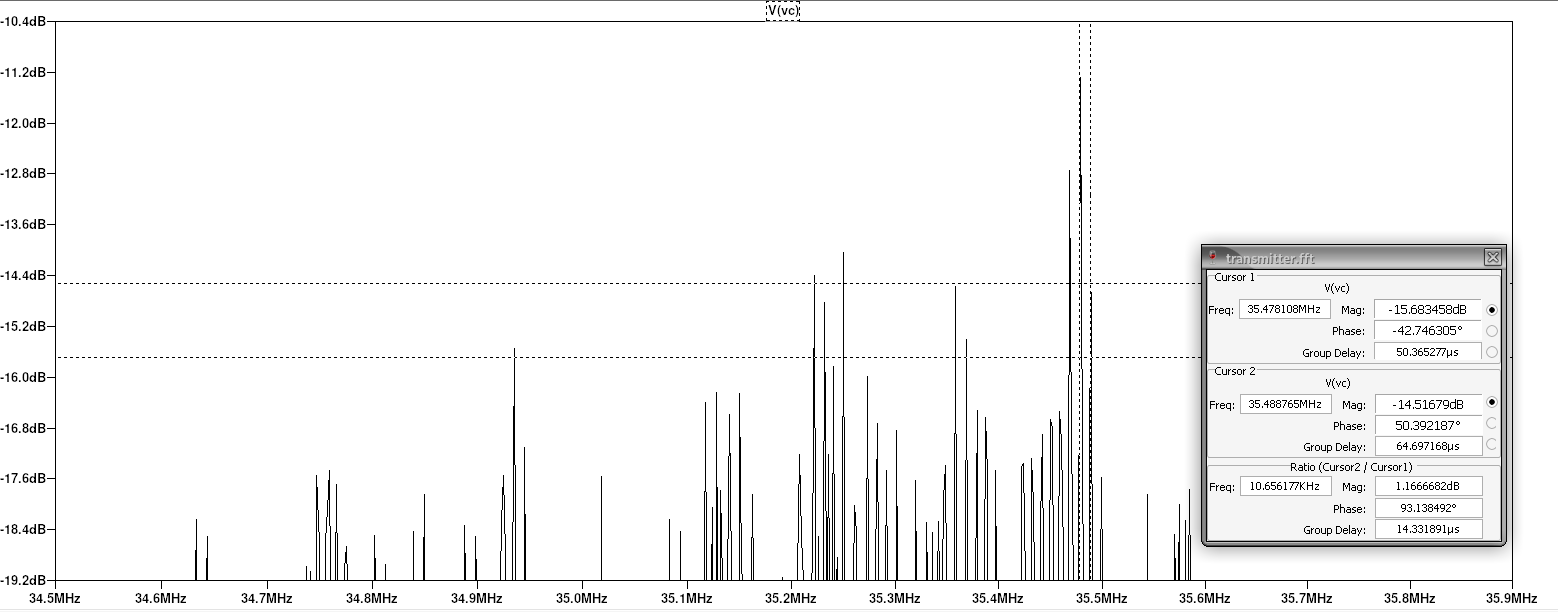
\includegraphics[scale=.8, width=.8\textwidth]{fft_vc_zoom}
    \caption{Simulaci\'on de la FFT de $V_C$ ampliada a la frecuencia de trabajo}
    \label{fig:sim_fft_zoom}
\end{figure}

\paragraph{Resultado de la pr\'actica} %CAPTURA DEL OSCILOSCOPIO Y MEDIDA DE CORRIENTE
\paragraph{}
En la parte práctica se comparan los resultados de la simulación con los resultados obtenidos en el circuito real. 
\paragraph{}
El circuito está fabricado en placa soldada de agujeros, la realizaci\'on de estas placas se muestra en la figura \ref{fig:exp_placa_tx}. Los resultados se miden con un osciloscopio en los mismos puntos de interés que en el apartado de simulación. Las figuras corresponden a capturas realizadas por el osciloscopio al tomar las medidas pertinentes.

\begin{figure}[h!]
    \centering
    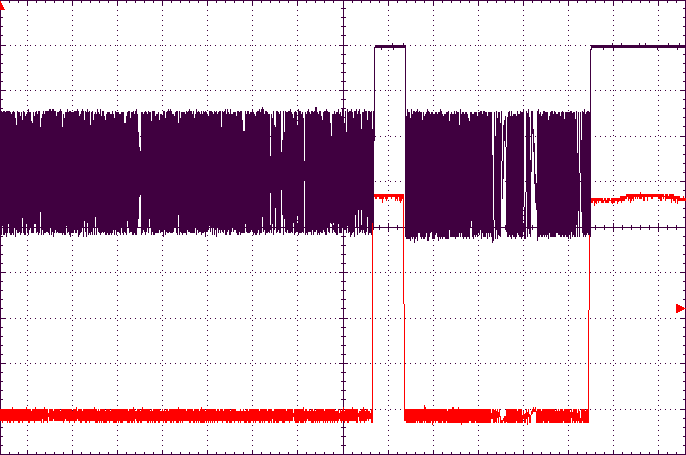
\includegraphics[scale=.6, width=.6\textwidth]{exp_tx}
    \caption{Experimental: captura de osciloscopio de $V_C$ modulada por $V_{digital}$}
    \label{fig:exp_vc_vdig}
\end{figure}

\begin{figure}[h!]
    \centering
    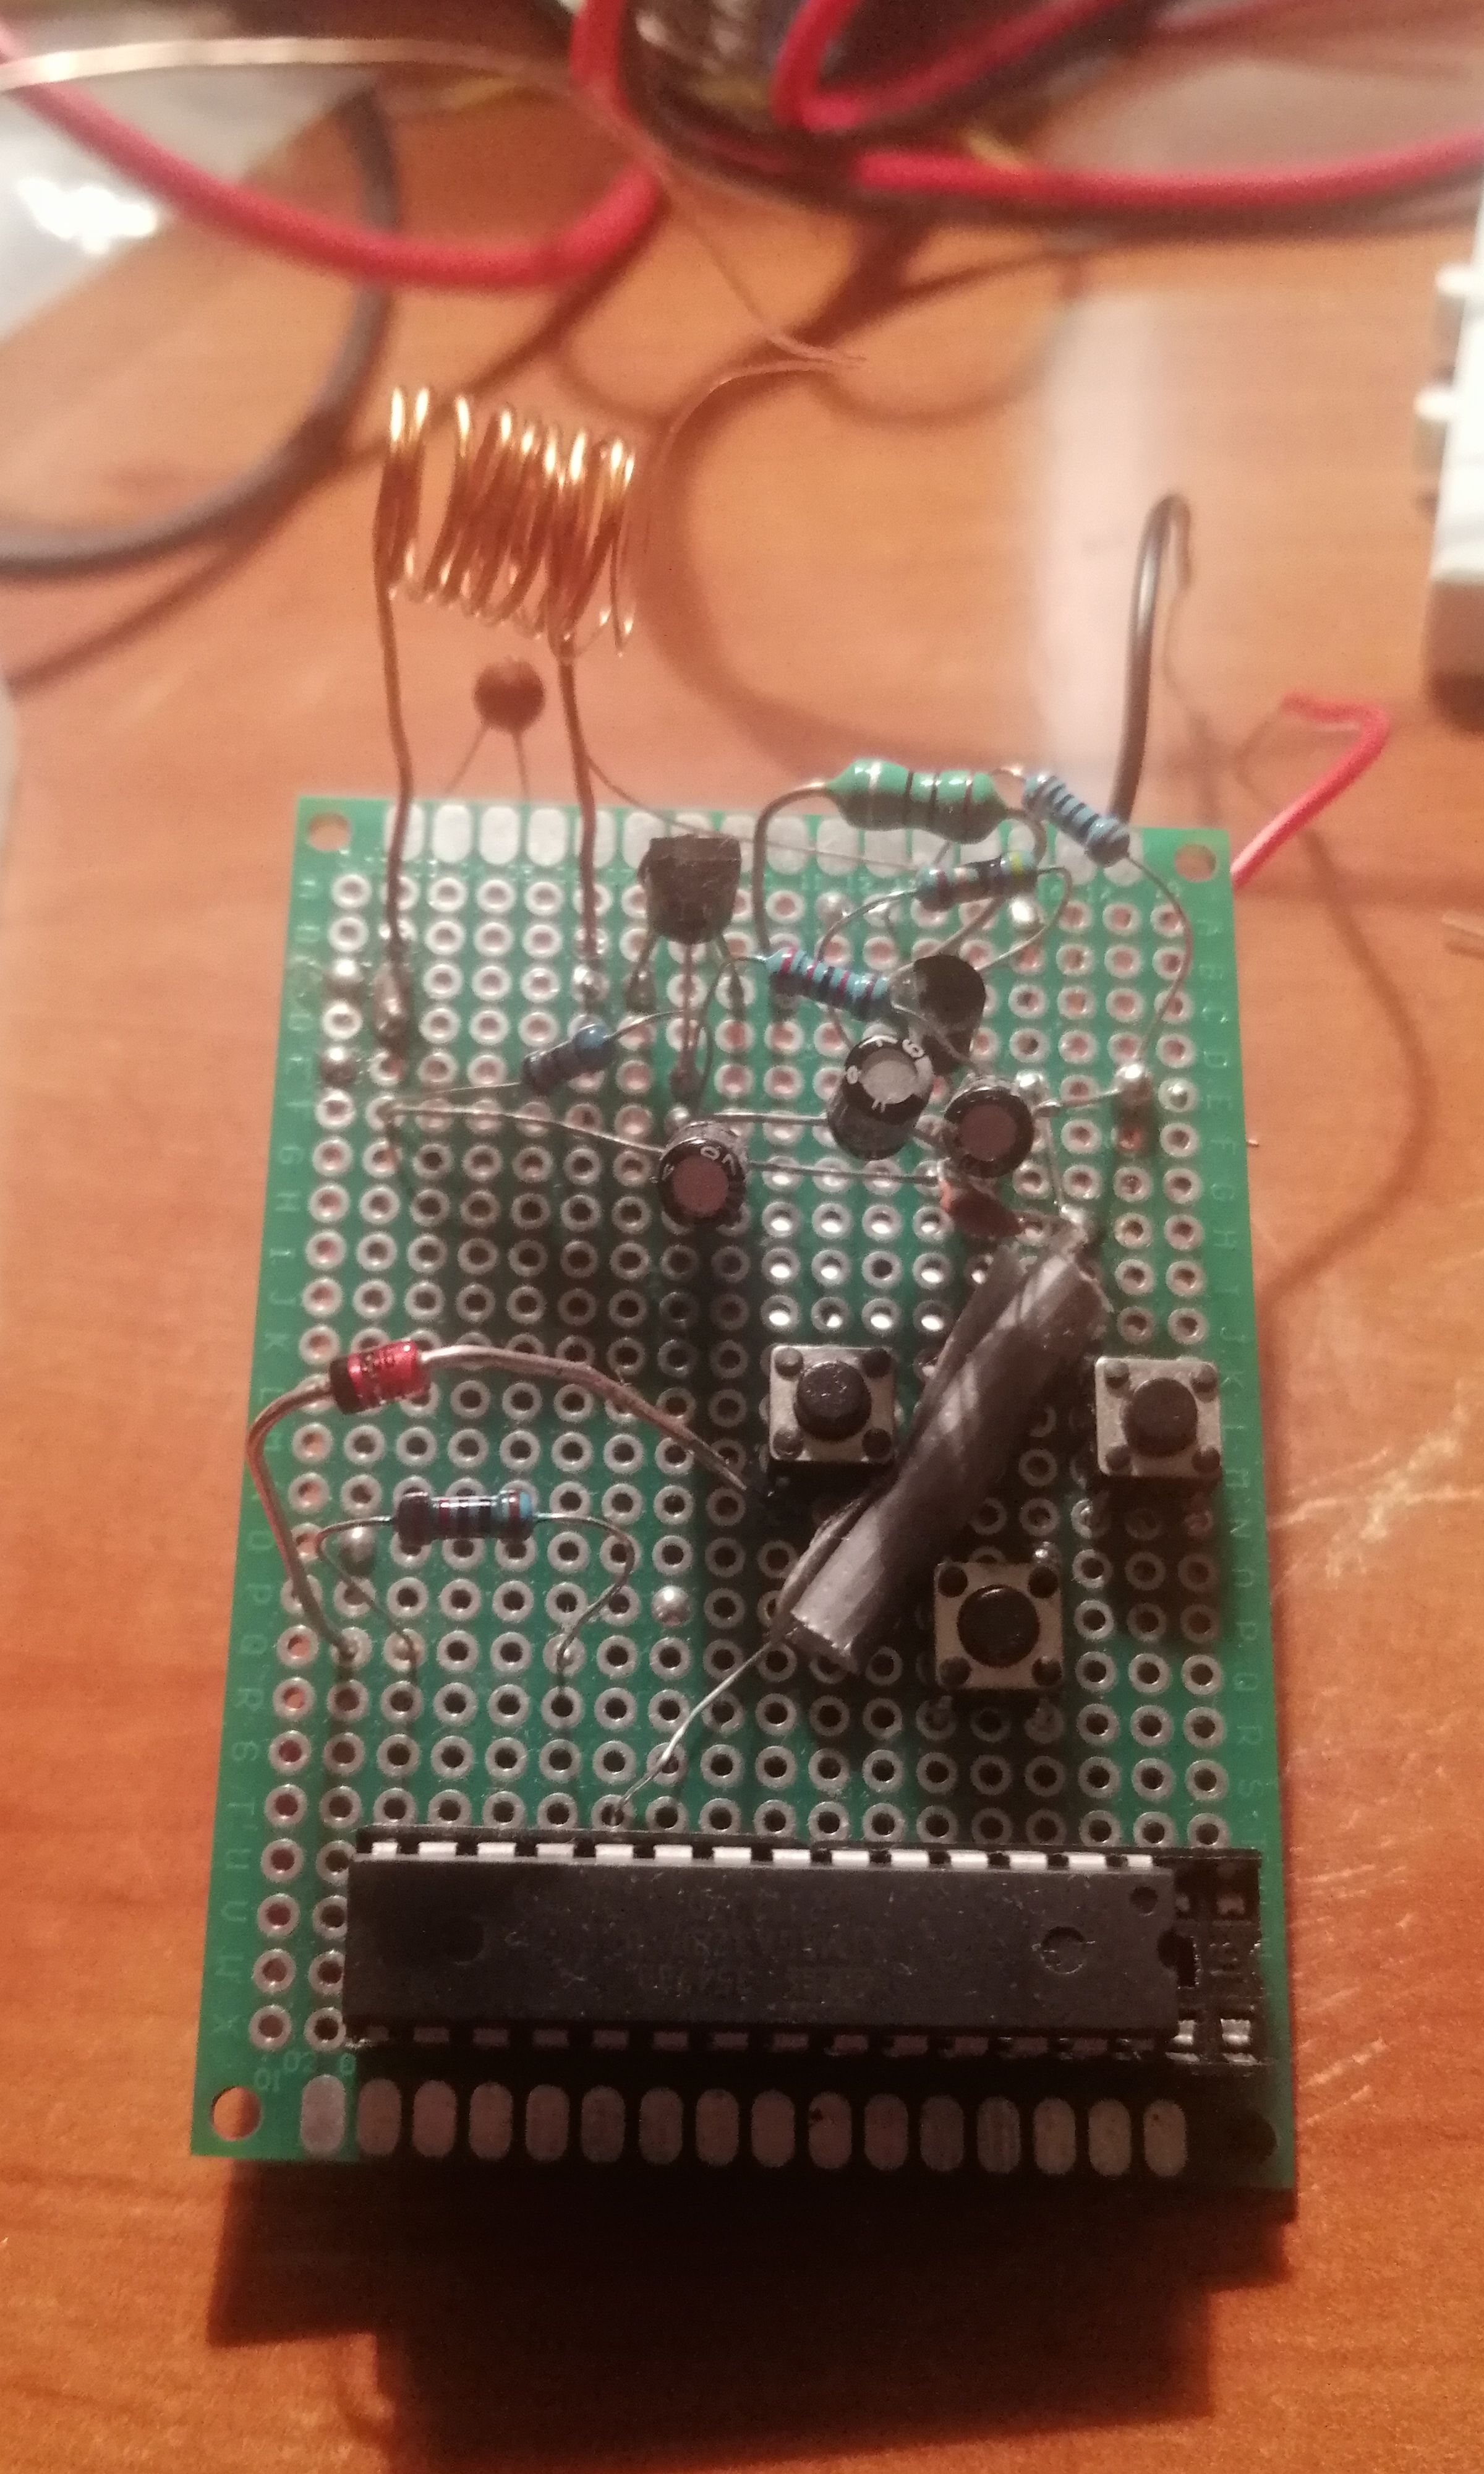
\includegraphics[scale=.3, width=.3\textwidth]{des_tx_real}
    \caption{Placa de transmisor soldada}
    \label{fig:exp_placa_tx}
\end{figure}

% \paragraph{Modulaci\'on de los canales mediante NE555}
% \paragraph{}
% La estrategia para la modulaci\'on reside en concepto de NE555 es un chip, el cual, configurado adecuadamente puede trabajar como un astable. Adem\'as, la frecuencia de oscilación del astable puede ser variada en función de los elementos de configuración. La idea es utilizar la señal proporcionada por el chip para cortar el oscilador según la frecuencia del NE555, realizando una mezcla de ambas señales y dando lugar a la señal modulada ASK. La mezcla se realiza por medio del transistor Q2 PNP, el cual trabaja en corte y saturación.
% \paragraph{}
% La configuraci\'on de astable para el chip NE555 viene dada en la datasheet del mismo, por lo que se sigue el modelo de esta configuraci\'on. El chip soporta un rango de tensiones de alimentaci\'on $4.5 < V_{CC} < 16$ \unit{\volt}, por lo que se ajusta a las condiciones del trabajo. Se realiza el diseño y el valor de los componentes siguiendo las siguientes ecuaciones proporcionadas por la hoja de datos:
% 
% \begin{align} 
%    \label{eq:freq}
%    Freq &= \frac{1.44}{(R_A + 2 \cdot R_B) \cdot C} \\
%    \label{eq:duty}
%    Duty &= \frac{1.44}{(R_A + 2 \cdot R_B)}
% \end{align}
% 
% Se requiere un ciclo de trabajo de aproximadamente $Duty \approx 0.5$ por lo que $R_B >> R_A$. La frecuencias de la onda cuadrada moduladora son de \SI{15}{\kilo\hertz} y \SI{3}{\kilo\hertz} para distintos valores de $R_B$. Estas frecuencias son alternadas mediante dos pulsadores los cuales conectan los dos distintos valores de $R_B$ al circuito tras ser accionados, generando as\'i dos distintos canales digitales. Cabe mencionar que $R_A$ no puede ser arbitrariamente pequeña, pues el el esquema eléctrico del chip que proporciona el fabricante, $R_A$ se conecta como resistencia de colector del transistor de \textit{DISCH}. Hacer $R_A$ más pequeño incurre en mayor consumo del chip en cada semiciclo.
% \paragraph{}
% Las frecuencias de modulación se eligen teniendo en cuenta: la facilidad de filtrado con respecto a las bajas frecuencias, los valores de $R_B$ y $R_A$, y la frecuencia de muestreo del ADC en el decodificador digital. Teniendo en cuenta estos parámetros, se calculan $R_A$ y $R_B$ con las ecuaciones.
% \paragraph{}
% En primer lugar, se selecciona $R_A$ para obtener un consumo razonable de descarga siguiendo la ecuaci\'on $I_{Disch} = \frac{V_{CC}-0.2}{R_A}$, un valor de $R_A = \SI{500}{\ohm}$ da lugar a $I_{Disch} = \SI{17.6}{\milli\ampere}$, lo cual es aceptable. En segundo lugar se debe fijar el ciclo de trabajo, si se hace $R_B = 10 \cdot R_A$ es una aproximaci\'on suficiente, ya que, mediante la ecuaci\'on \ref{eq:duty} queda $Duty = 0.476 \approx 0.5$. Por \'ultimo se fijan las frecuencias de modulaci\'on mediante la ecuaci\'on \ref{eq:freq}, lo cual nos fija un valor de $C$. Al tener dos diferentes canales con dos valores de frecuencia y $R_B$, se obtiene el siguiente sistema de ecuaciones para obtener el valor de $C$:
% \begin{align*} 
%    Freq_1 &= \frac{1.44}{(R_A + 2 \cdot R_{B1}) \cdot C} \\
%    Freq_2 &= \frac{1.44}{(R_A + 2 \cdot R_{B2}) \cdot C} \\
% \end{align*}
% 
% siendo  $Freq_1= \SI{15}{\kilo\hertz}$ $Freq_2=\SI{3}{\kilo\hertz}$ $R_{B1}=\SI{10}{\kilo\ohm}$ $R_{B2}=\SI{5}{\kilo\ohm}$, el valor de $C$ como resultado es $C \approx \SI{6.8}{\nano\farad}$



